% Options for packages loaded elsewhere
\PassOptionsToPackage{unicode}{hyperref}
\PassOptionsToPackage{hyphens}{url}
%
\documentclass[
  ignorenonframetext,
]{beamer}
\usepackage{pgfpages}
\setbeamertemplate{caption}[numbered]
\setbeamertemplate{caption label separator}{: }
\setbeamercolor{caption name}{fg=normal text.fg}
\beamertemplatenavigationsymbolsempty
% Prevent slide breaks in the middle of a paragraph
\widowpenalties 1 10000
\raggedbottom
\setbeamertemplate{part page}{
  \centering
  \begin{beamercolorbox}[sep=16pt,center]{part title}
    \usebeamerfont{part title}\insertpart\par
  \end{beamercolorbox}
}
\setbeamertemplate{section page}{
  \centering
  \begin{beamercolorbox}[sep=12pt,center]{part title}
    \usebeamerfont{section title}\insertsection\par
  \end{beamercolorbox}
}
\setbeamertemplate{subsection page}{
  \centering
  \begin{beamercolorbox}[sep=8pt,center]{part title}
    \usebeamerfont{subsection title}\insertsubsection\par
  \end{beamercolorbox}
}
\AtBeginPart{
  \frame{\partpage}
}
\AtBeginSection{
  \ifbibliography
  \else
    \frame{\sectionpage}
  \fi
}
\AtBeginSubsection{
  \frame{\subsectionpage}
}
\usepackage{amsmath,amssymb}
\usepackage{iftex}
\ifPDFTeX
  \usepackage[T1]{fontenc}
  \usepackage[utf8]{inputenc}
  \usepackage{textcomp} % provide euro and other symbols
\else % if luatex or xetex
  \usepackage{unicode-math} % this also loads fontspec
  \defaultfontfeatures{Scale=MatchLowercase}
  \defaultfontfeatures[\rmfamily]{Ligatures=TeX,Scale=1}
\fi
\usepackage{lmodern}
\usetheme[]{CambridgeUS}
\usecolortheme{seahorse}
\usefonttheme{structurebold}
\ifPDFTeX\else
  % xetex/luatex font selection
\fi
% Use upquote if available, for straight quotes in verbatim environments
\IfFileExists{upquote.sty}{\usepackage{upquote}}{}
\IfFileExists{microtype.sty}{% use microtype if available
  \usepackage[]{microtype}
  \UseMicrotypeSet[protrusion]{basicmath} % disable protrusion for tt fonts
}{}
\makeatletter
\@ifundefined{KOMAClassName}{% if non-KOMA class
  \IfFileExists{parskip.sty}{%
    \usepackage{parskip}
  }{% else
    \setlength{\parindent}{0pt}
    \setlength{\parskip}{6pt plus 2pt minus 1pt}}
}{% if KOMA class
  \KOMAoptions{parskip=half}}
\makeatother
\usepackage{xcolor}
\newif\ifbibliography
\usepackage{color}
\usepackage{fancyvrb}
\newcommand{\VerbBar}{|}
\newcommand{\VERB}{\Verb[commandchars=\\\{\}]}
\DefineVerbatimEnvironment{Highlighting}{Verbatim}{commandchars=\\\{\}}
% Add ',fontsize=\small' for more characters per line
\usepackage{framed}
\definecolor{shadecolor}{RGB}{248,248,248}
\newenvironment{Shaded}{\begin{snugshade}}{\end{snugshade}}
\newcommand{\AlertTok}[1]{\textcolor[rgb]{0.94,0.16,0.16}{#1}}
\newcommand{\AnnotationTok}[1]{\textcolor[rgb]{0.56,0.35,0.01}{\textbf{\textit{#1}}}}
\newcommand{\AttributeTok}[1]{\textcolor[rgb]{0.13,0.29,0.53}{#1}}
\newcommand{\BaseNTok}[1]{\textcolor[rgb]{0.00,0.00,0.81}{#1}}
\newcommand{\BuiltInTok}[1]{#1}
\newcommand{\CharTok}[1]{\textcolor[rgb]{0.31,0.60,0.02}{#1}}
\newcommand{\CommentTok}[1]{\textcolor[rgb]{0.56,0.35,0.01}{\textit{#1}}}
\newcommand{\CommentVarTok}[1]{\textcolor[rgb]{0.56,0.35,0.01}{\textbf{\textit{#1}}}}
\newcommand{\ConstantTok}[1]{\textcolor[rgb]{0.56,0.35,0.01}{#1}}
\newcommand{\ControlFlowTok}[1]{\textcolor[rgb]{0.13,0.29,0.53}{\textbf{#1}}}
\newcommand{\DataTypeTok}[1]{\textcolor[rgb]{0.13,0.29,0.53}{#1}}
\newcommand{\DecValTok}[1]{\textcolor[rgb]{0.00,0.00,0.81}{#1}}
\newcommand{\DocumentationTok}[1]{\textcolor[rgb]{0.56,0.35,0.01}{\textbf{\textit{#1}}}}
\newcommand{\ErrorTok}[1]{\textcolor[rgb]{0.64,0.00,0.00}{\textbf{#1}}}
\newcommand{\ExtensionTok}[1]{#1}
\newcommand{\FloatTok}[1]{\textcolor[rgb]{0.00,0.00,0.81}{#1}}
\newcommand{\FunctionTok}[1]{\textcolor[rgb]{0.13,0.29,0.53}{\textbf{#1}}}
\newcommand{\ImportTok}[1]{#1}
\newcommand{\InformationTok}[1]{\textcolor[rgb]{0.56,0.35,0.01}{\textbf{\textit{#1}}}}
\newcommand{\KeywordTok}[1]{\textcolor[rgb]{0.13,0.29,0.53}{\textbf{#1}}}
\newcommand{\NormalTok}[1]{#1}
\newcommand{\OperatorTok}[1]{\textcolor[rgb]{0.81,0.36,0.00}{\textbf{#1}}}
\newcommand{\OtherTok}[1]{\textcolor[rgb]{0.56,0.35,0.01}{#1}}
\newcommand{\PreprocessorTok}[1]{\textcolor[rgb]{0.56,0.35,0.01}{\textit{#1}}}
\newcommand{\RegionMarkerTok}[1]{#1}
\newcommand{\SpecialCharTok}[1]{\textcolor[rgb]{0.81,0.36,0.00}{\textbf{#1}}}
\newcommand{\SpecialStringTok}[1]{\textcolor[rgb]{0.31,0.60,0.02}{#1}}
\newcommand{\StringTok}[1]{\textcolor[rgb]{0.31,0.60,0.02}{#1}}
\newcommand{\VariableTok}[1]{\textcolor[rgb]{0.00,0.00,0.00}{#1}}
\newcommand{\VerbatimStringTok}[1]{\textcolor[rgb]{0.31,0.60,0.02}{#1}}
\newcommand{\WarningTok}[1]{\textcolor[rgb]{0.56,0.35,0.01}{\textbf{\textit{#1}}}}
\usepackage{longtable,booktabs,array}
\usepackage{calc} % for calculating minipage widths
\usepackage{caption}
% Make caption package work with longtable
\makeatletter
\def\fnum@table{\tablename~\thetable}
\makeatother
\usepackage{graphicx}
\makeatletter
\def\maxwidth{\ifdim\Gin@nat@width>\linewidth\linewidth\else\Gin@nat@width\fi}
\def\maxheight{\ifdim\Gin@nat@height>\textheight\textheight\else\Gin@nat@height\fi}
\makeatother
% Scale images if necessary, so that they will not overflow the page
% margins by default, and it is still possible to overwrite the defaults
% using explicit options in \includegraphics[width, height, ...]{}
\setkeys{Gin}{width=\maxwidth,height=\maxheight,keepaspectratio}
% Set default figure placement to htbp
\makeatletter
\def\fps@figure{htbp}
\makeatother
\setlength{\emergencystretch}{3em} % prevent overfull lines
\providecommand{\tightlist}{%
  \setlength{\itemsep}{0pt}\setlength{\parskip}{0pt}}
\setcounter{secnumdepth}{-\maxdimen} % remove section numbering
\ifLuaTeX
  \usepackage{selnolig}  % disable illegal ligatures
\fi
\usepackage{bookmark}
\IfFileExists{xurl.sty}{\usepackage{xurl}}{} % add URL line breaks if available
\urlstyle{same}
\hypersetup{
  pdftitle={Loops, Prediction, and Regression},
  pdfauthor={Prof.~Weldzius},
  hidelinks,
  pdfcreator={LaTeX via pandoc}}

\title{Loops, Prediction, and Regression}
\subtitle{PSC7475: Week 5}
\author{Prof.~Weldzius}
\date{Slides Updated: 2025-03-10}
\institute{Villanova University}

\begin{document}
\frame{\titlepage}

\begin{frame}{2016 US Presidential Election}
\phantomsection\label{us-presidential-election}
\begin{center}
  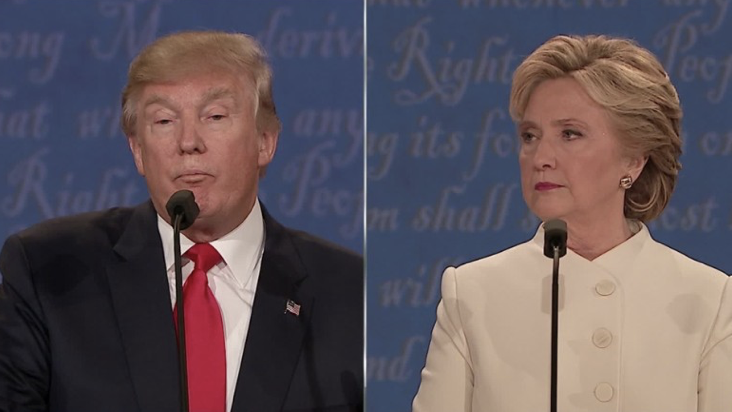
\includegraphics[width=.5\textwidth]{figs/2016election.png}
  \end{center} \pause

\begin{itemize}
\tightlist
\item
  2016 election popular vote: \pause

  \begin{itemize}
  \tightlist
  \item
    Clinton: 65,853,516 (48.2\%)
  \item
    Trump: 62,984,825 (46.1\%) \pause
  \end{itemize}
\item
  Why did Trump win? \textbf{Electoral college}

  \begin{itemize}
  \tightlist
  \item
    Trump: 304, Clinton: 227 \pause
  \end{itemize}
\item
  Election determined by 77,744 votes (margins in WI, MI, PA)

  \begin{itemize}
  \tightlist
  \item
    0.056\% of the electorate (\textasciitilde136million)
  \end{itemize}
\end{itemize}
\end{frame}

\begin{frame}{Predicting US Presidential Elections}
\phantomsection\label{predicting-us-presidential-elections}
\pause

\begin{itemize}
\tightlist
\item
  \textbf{Electoral college system} \pause

  \begin{itemize}
  \tightlist
  \item
    Must win an absolute majority of 538 electoral votes \pause
  \item
    538 = 435 (House of Representatives) + 100 (Senators) + 3 (DC)
    \pause
  \item
    Must win at least 270 votes \pause
  \item
    nobody wins an absolute majority \(\rightsquigarrow\) House vote
    \pause
  \end{itemize}
\item
  Must predict winner of each state \pause
\end{itemize}

\begin{center}
  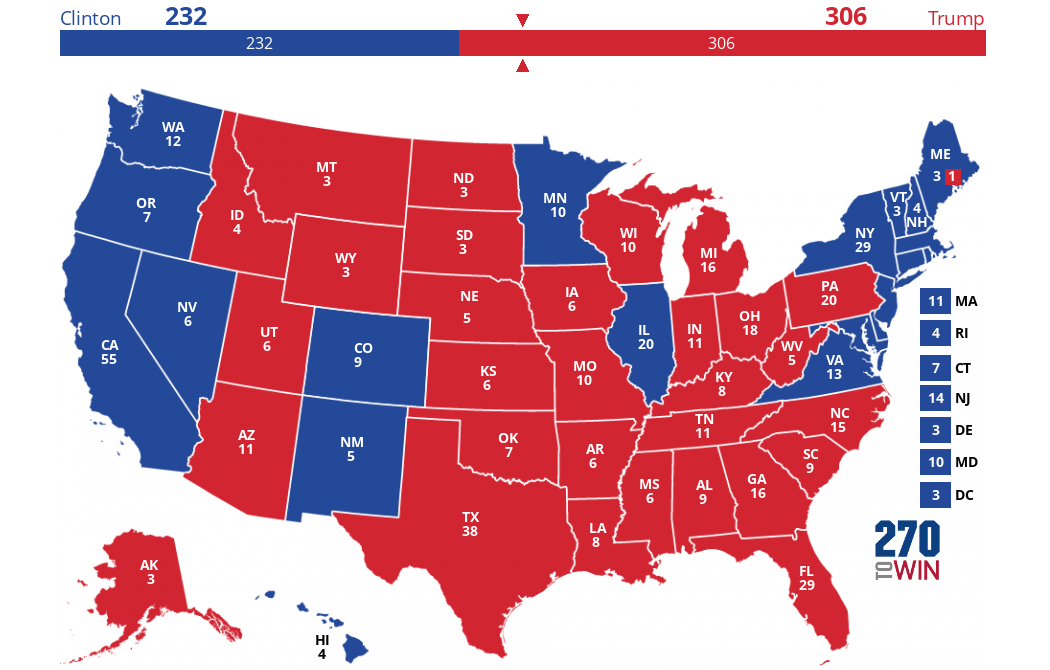
\includegraphics[width=.6\textwidth]{figs/2016electcol.png}
  \end{center}
\end{frame}

\begin{frame}{Prediction strategy}
\phantomsection\label{prediction-strategy}
\pause

\begin{itemize}
\item
  Predict state-level support for each candidate using polls \pause
\item
  Allocate electoral college votes of that state to its predicted winner
  \pause
\item
  Aggregate EC votes across states to determine the predicted winner
  \pause
\item
  Coding strategy: \pause

  \begin{enumerate}
  \tightlist
  \item
    For each state, subset to polls within that state \pause
  \item
    Further subset the latest polls \pause
  \item
    Average the latest polls to estimate support for each candidate
    \pause
  \item
    Allocate the electoral votes to the candidate who has greatest
    support \pause
  \item
    Repeat this for all states and aggregate the electoral votes \pause 
  \end{enumerate}
\item
  Sounds like a lot of subsets, ugh\ldots{}
\end{itemize}
\end{frame}

\begin{frame}[fragile,t]{Multiplication}
\phantomsection\label{multiplication}
\pause

\begin{itemize}
\tightlist
\item
  Let's create a new variable that multiples each value in a vector by
  2: \pause

  \begin{itemize}
  \tightlist
  \item
    Easy in R: \texttt{values\ *\ 2} \pause
  \item
    Pretend you didn't know this approach
  \end{itemize}
\end{itemize}
\end{frame}

\begin{frame}[fragile,t]{Multiplication}
\phantomsection\label{multiplication-1}
\footnotesize

\begin{Shaded}
\begin{Highlighting}[]
\NormalTok{values }\OtherTok{\textless{}{-}} \FunctionTok{c}\NormalTok{(}\DecValTok{2}\NormalTok{,}\DecValTok{4}\NormalTok{,}\DecValTok{6}\NormalTok{)}
\end{Highlighting}
\end{Shaded}
\end{frame}

\begin{frame}[fragile,t]{Multiplication}
\phantomsection\label{multiplication-2}
\footnotesize

\begin{Shaded}
\begin{Highlighting}[]
\NormalTok{values }\OtherTok{\textless{}{-}} \FunctionTok{c}\NormalTok{(}\DecValTok{2}\NormalTok{,}\DecValTok{4}\NormalTok{,}\DecValTok{6}\NormalTok{)}

\DocumentationTok{\#\# number of values}
\NormalTok{n }\OtherTok{\textless{}{-}} \FunctionTok{length}\NormalTok{(values)}
\end{Highlighting}
\end{Shaded}
\end{frame}

\begin{frame}[fragile,t]{Multiplication}
\phantomsection\label{multiplication-3}
\footnotesize

\begin{Shaded}
\begin{Highlighting}[]
\NormalTok{values }\OtherTok{\textless{}{-}} \FunctionTok{c}\NormalTok{(}\DecValTok{2}\NormalTok{,}\DecValTok{4}\NormalTok{,}\DecValTok{6}\NormalTok{)}

\DocumentationTok{\#\# number of values}
\NormalTok{n }\OtherTok{\textless{}{-}} \FunctionTok{length}\NormalTok{(values)}

\DocumentationTok{\#\# create container to hold results}
\NormalTok{results }\OtherTok{\textless{}{-}} \FunctionTok{rep}\NormalTok{(}\ConstantTok{NA}\NormalTok{, }\AttributeTok{times =}\NormalTok{ n)}
\end{Highlighting}
\end{Shaded}
\end{frame}

\begin{frame}[fragile,t]{Multiplication}
\phantomsection\label{multiplication-4}
\footnotesize

\begin{Shaded}
\begin{Highlighting}[]
\NormalTok{values }\OtherTok{\textless{}{-}} \FunctionTok{c}\NormalTok{(}\DecValTok{2}\NormalTok{,}\DecValTok{4}\NormalTok{,}\DecValTok{6}\NormalTok{)}

\DocumentationTok{\#\# number of values}
\NormalTok{n }\OtherTok{\textless{}{-}} \FunctionTok{length}\NormalTok{(values)}

\DocumentationTok{\#\# create container to hold results}
\NormalTok{results }\OtherTok{\textless{}{-}} \FunctionTok{rep}\NormalTok{(}\ConstantTok{NA}\NormalTok{, }\AttributeTok{times =}\NormalTok{ n)}

\DocumentationTok{\#\# multiply each value by 2}
\NormalTok{results[}\DecValTok{1}\NormalTok{] }\OtherTok{\textless{}{-}}\NormalTok{ values[}\DecValTok{1}\NormalTok{] }\SpecialCharTok{*} \DecValTok{2}
\NormalTok{results[}\DecValTok{2}\NormalTok{] }\OtherTok{\textless{}{-}}\NormalTok{ values[}\DecValTok{2}\NormalTok{] }\SpecialCharTok{*} \DecValTok{2}
\NormalTok{results[}\DecValTok{3}\NormalTok{] }\OtherTok{\textless{}{-}}\NormalTok{ values[}\DecValTok{3}\NormalTok{] }\SpecialCharTok{*} \DecValTok{2}
\end{Highlighting}
\end{Shaded}
\end{frame}

\begin{frame}[fragile,t]{Multiplication}
\phantomsection\label{multiplication-5}
\footnotesize

\begin{Shaded}
\begin{Highlighting}[]
\NormalTok{values }\OtherTok{\textless{}{-}} \FunctionTok{c}\NormalTok{(}\DecValTok{2}\NormalTok{,}\DecValTok{4}\NormalTok{,}\DecValTok{6}\NormalTok{)}

\DocumentationTok{\#\# number of values}
\NormalTok{n }\OtherTok{\textless{}{-}} \FunctionTok{length}\NormalTok{(values)}

\DocumentationTok{\#\# create container to hold results}
\NormalTok{results }\OtherTok{\textless{}{-}} \FunctionTok{rep}\NormalTok{(}\ConstantTok{NA}\NormalTok{, }\AttributeTok{times =}\NormalTok{ n)}

\DocumentationTok{\#\# multiply each value by 2}
\NormalTok{results[}\DecValTok{1}\NormalTok{] }\OtherTok{\textless{}{-}}\NormalTok{ values[}\DecValTok{1}\NormalTok{] }\SpecialCharTok{*} \DecValTok{2}
\NormalTok{results[}\DecValTok{2}\NormalTok{] }\OtherTok{\textless{}{-}}\NormalTok{ values[}\DecValTok{2}\NormalTok{] }\SpecialCharTok{*} \DecValTok{2}
\NormalTok{results[}\DecValTok{3}\NormalTok{] }\OtherTok{\textless{}{-}}\NormalTok{ values[}\DecValTok{3}\NormalTok{] }\SpecialCharTok{*} \DecValTok{2}

\NormalTok{results}
\end{Highlighting}
\end{Shaded}

\begin{verbatim}
## [1]  4  8 12
\end{verbatim}
\end{frame}

\begin{frame}[fragile]{Loops in R}
\phantomsection\label{loops-in-r}
\pause

\begin{itemize}
\tightlist
\item
  What if you had more values? Not efficient! \pause

  \begin{itemize}
  \tightlist
  \item
    \textbf{for loop}: a way to iteratively execute the same code
    multiple times. \pause
  \end{itemize}
\item
  Basic structure: \pause
\end{itemize}

\small

\begin{Shaded}
\begin{Highlighting}[]
\ControlFlowTok{for}\NormalTok{ (i }\ControlFlowTok{in}\NormalTok{ X) \{}
\NormalTok{  expression1}
\NormalTok{  expression2}
\NormalTok{  ...}
\NormalTok{  expression3}
\NormalTok{\}}
\end{Highlighting}
\end{Shaded}

\pause

\begin{itemize}
\tightlist
\item
  Elements of a loop: \pause

  \begin{itemize}
  \tightlist
  \item
    \texttt{i}: counter (can use any name) \pause
  \item
    \texttt{X}: vector containing a set of ordered values the counter
    takes \pause
  \item
    \texttt{expression}: a set of expressions that will be repeatedly
    evaluated. \pause
  \item
    \texttt{\{\ \}}: curly braces to define beginning and end of the
    loop. \pause
  \end{itemize}
\item
  Indentation is important for readability of the code.
\end{itemize}
\end{frame}

\begin{frame}[fragile]{Loop example:}
\phantomsection\label{loop-example}
\small

\begin{Shaded}
\begin{Highlighting}[]
\NormalTok{values }\OtherTok{\textless{}{-}} \FunctionTok{c}\NormalTok{(}\DecValTok{2}\NormalTok{,}\DecValTok{4}\NormalTok{,}\DecValTok{6}\NormalTok{)}
\NormalTok{n }\OtherTok{\textless{}{-}} \FunctionTok{length}\NormalTok{(values)}
\NormalTok{results }\OtherTok{\textless{}{-}} \FunctionTok{rep}\NormalTok{(}\ConstantTok{NA}\NormalTok{, }\AttributeTok{times =}\NormalTok{ n)}

\DocumentationTok{\#\# begin loop}
\ControlFlowTok{for}\NormalTok{ (i }\ControlFlowTok{in} \DecValTok{1}\SpecialCharTok{:}\NormalTok{n) \{}
\NormalTok{  results[i] }\OtherTok{\textless{}{-}}\NormalTok{ values[i] }\SpecialCharTok{*} \DecValTok{2}
  \FunctionTok{print}\NormalTok{(}\FunctionTok{str\_c}\NormalTok{(values[i], }\StringTok{" times 2 is equal to "}\NormalTok{, results[i]))}
\NormalTok{\}}
\end{Highlighting}
\end{Shaded}

\begin{verbatim}
## [1] "2 times 2 is equal to 4"
## [1] "4 times 2 is equal to 8"
## [1] "6 times 2 is equal to 12"
\end{verbatim}
\end{frame}

\begin{frame}[fragile]{2016 polling prediction}
\phantomsection\label{polling-prediction}
\begin{itemize}
\tightlist
\item
  Election data: \texttt{pres.csv}
\end{itemize}

\footnotesize

\begin{longtable}[]{@{}
  >{\raggedright\arraybackslash}p{(\columnwidth - 2\tabcolsep) * \real{0.1495}}
  >{\raggedright\arraybackslash}p{(\columnwidth - 2\tabcolsep) * \real{0.8505}}@{}}
\toprule\noalign{}
\begin{minipage}[b]{\linewidth}\raggedright
Name
\end{minipage} & \begin{minipage}[b]{\linewidth}\raggedright
Description
\end{minipage} \\
\midrule\noalign{}
\endhead
\texttt{state\_abb} & abbreviated name of state \\
\texttt{clinton} & Clinton's vote share (percentage) \\
\texttt{trump} & Trump's vote share (percentage) \\
\bottomrule\noalign{}
\end{longtable}

\begin{itemize}
\tightlist
\item
  Polling data \texttt{polls16.csv}
\end{itemize}

\footnotesize

\begin{longtable}[]{@{}
  >{\raggedright\arraybackslash}p{(\columnwidth - 2\tabcolsep) * \real{0.1495}}
  >{\raggedright\arraybackslash}p{(\columnwidth - 2\tabcolsep) * \real{0.8505}}@{}}
\toprule\noalign{}
\begin{minipage}[b]{\linewidth}\raggedright
Name
\end{minipage} & \begin{minipage}[b]{\linewidth}\raggedright
Description
\end{minipage} \\
\midrule\noalign{}
\endhead
\texttt{state} & abbreviated name of state in which polls was
conducted \\
\texttt{middate} & middate of the period when polls was conducted \\
\texttt{daysleft} & number of days between middate and election day \\
\texttt{pollster} & name of organization conducting poll \\
\texttt{clinton} & predicted support for Clinton (percentage) \\
\texttt{trump} & predicted support for Trump (percentage) \\
\bottomrule\noalign{}
\end{longtable}
\end{frame}

\begin{frame}[fragile]{Some preprocessing}
\phantomsection\label{some-preprocessing}
\begin{Shaded}
\begin{Highlighting}[]
\DocumentationTok{\#\# download; don\textquotesingle{}t forget to setwd()}
\NormalTok{pres16 }\OtherTok{\textless{}{-}} \FunctionTok{read\_csv}\NormalTok{(}\StringTok{"../data/pres2016.csv"}\NormalTok{)}
\NormalTok{polls16 }\OtherTok{\textless{}{-}} \FunctionTok{read\_csv}\NormalTok{(}\StringTok{"../data/polls2016.csv"}\NormalTok{)}

\DocumentationTok{\#\# calculate Trump\textquotesingle{}s margin of victory}
\NormalTok{polls16 }\OtherTok{\textless{}{-}}\NormalTok{ polls16 }\SpecialCharTok{\%\textgreater{}\%}
  \FunctionTok{mutate}\NormalTok{(}\AttributeTok{margin =}\NormalTok{ Trump }\SpecialCharTok{{-}}\NormalTok{ Clinton)}
\NormalTok{pres16 }\OtherTok{\textless{}{-}}\NormalTok{ pres16 }\SpecialCharTok{\%\textgreater{}\%}
  \FunctionTok{mutate}\NormalTok{(}\AttributeTok{margin =}\NormalTok{ Trump }\SpecialCharTok{{-}}\NormalTok{ Clinton)}
\end{Highlighting}
\end{Shaded}
\end{frame}

\begin{frame}[fragile]{What does the data look like?}
\phantomsection\label{what-does-the-data-look-like}
\footnotesize

\begin{Shaded}
\begin{Highlighting}[]
\FunctionTok{head}\NormalTok{(polls16)}
\end{Highlighting}
\end{Shaded}

\begin{verbatim}
## # A tibble: 6 x 8
##      id state Clinton Trump days_to_election electoral_votes
##   <dbl> <chr>   <dbl> <dbl>            <dbl>           <dbl>
## 1 26255 TX         38    41               24              38
## 2 26253 WI         48    44               23              10
## 3 26252 VA         54    41               23              13
## 4 26251 NV         47    40               19               6
## 5 26250 TX         46    48               23              38
## 6 26249 NH         50    43               23               4
## # i 2 more variables: population <chr>, margin <dbl>
\end{verbatim}
\end{frame}

\begin{frame}[fragile,t]{Poll prediction for each state}
\phantomsection\label{poll-prediction-for-each-state}
\footnotesize

\begin{Shaded}
\begin{Highlighting}[]
\DocumentationTok{\#\# place holder}
\NormalTok{poll.pred }\OtherTok{\textless{}{-}} \FunctionTok{rep}\NormalTok{(}\ConstantTok{NA}\NormalTok{, }\DecValTok{51}\NormalTok{)}

\DocumentationTok{\#\# get list of unique state names to iterate over}
\NormalTok{state\_names }\OtherTok{\textless{}{-}} \FunctionTok{unique}\NormalTok{(polls16}\SpecialCharTok{$}\NormalTok{state)}

\DocumentationTok{\#\# add labels to place holder}
\FunctionTok{names}\NormalTok{(poll.pred) }\OtherTok{\textless{}{-}}\NormalTok{ state\_names}
\end{Highlighting}
\end{Shaded}
\end{frame}

\begin{frame}[fragile,t]{Poll prediction for each state}
\phantomsection\label{poll-prediction-for-each-state-1}
\footnotesize

\begin{Shaded}
\begin{Highlighting}[]
\ControlFlowTok{for}\NormalTok{ (i }\ControlFlowTok{in} \FunctionTok{seq\_along}\NormalTok{(state\_names)) \{}
\end{Highlighting}
\end{Shaded}
\end{frame}

\begin{frame}[fragile,t]{Poll prediction for each state}
\phantomsection\label{poll-prediction-for-each-state-2}
\footnotesize

\begin{Shaded}
\begin{Highlighting}[]
\ControlFlowTok{for}\NormalTok{ (i }\ControlFlowTok{in} \FunctionTok{seq\_along}\NormalTok{(state\_names)) \{}
  \DocumentationTok{\#\# subset the ith state}
\NormalTok{  state.data }\OtherTok{\textless{}{-}}\NormalTok{ polls16 }\SpecialCharTok{\%\textgreater{}\%}
    \FunctionTok{filter}\NormalTok{(state }\SpecialCharTok{==}\NormalTok{ state\_names[i])}
\end{Highlighting}
\end{Shaded}
\end{frame}

\begin{frame}[fragile,t]{Poll prediction for each state}
\phantomsection\label{poll-prediction-for-each-state-3}
\footnotesize

\begin{Shaded}
\begin{Highlighting}[]
\ControlFlowTok{for}\NormalTok{ (i }\ControlFlowTok{in} \FunctionTok{seq\_along}\NormalTok{(state\_names)) \{}
  \DocumentationTok{\#\# subset the ith state}
\NormalTok{  state.data }\OtherTok{\textless{}{-}}\NormalTok{ polls16 }\SpecialCharTok{\%\textgreater{}\%}
    \FunctionTok{filter}\NormalTok{(state }\SpecialCharTok{==}\NormalTok{ state\_names[i])}
  
  \DocumentationTok{\#\# pull out the closest date (minimum days to election)}
\NormalTok{  min\_days }\OtherTok{\textless{}{-}} \FunctionTok{min}\NormalTok{(state.data}\SpecialCharTok{$}\NormalTok{days\_to\_election)}
\end{Highlighting}
\end{Shaded}
\end{frame}

\begin{frame}[fragile,t]{Poll prediction for each state}
\phantomsection\label{poll-prediction-for-each-state-4}
\footnotesize

\begin{Shaded}
\begin{Highlighting}[]
\ControlFlowTok{for}\NormalTok{ (i }\ControlFlowTok{in} \FunctionTok{seq\_along}\NormalTok{(state\_names)) \{}
  \DocumentationTok{\#\# subset the ith state}
\NormalTok{  state.data }\OtherTok{\textless{}{-}}\NormalTok{ polls16 }\SpecialCharTok{\%\textgreater{}\%}
    \FunctionTok{filter}\NormalTok{(state }\SpecialCharTok{==}\NormalTok{ state\_names[i])}
  
  \DocumentationTok{\#\# pull out the closest date (minimum days to election)}
\NormalTok{  min\_days }\OtherTok{\textless{}{-}} \FunctionTok{min}\NormalTok{(state.data}\SpecialCharTok{$}\NormalTok{days\_to\_election)}
  
  \DocumentationTok{\#\# subset only the latest polls within the state}
\NormalTok{  state.data }\OtherTok{\textless{}{-}}\NormalTok{ state.data }\SpecialCharTok{\%\textgreater{}\%}
    \FunctionTok{filter}\NormalTok{(days\_to\_election }\SpecialCharTok{==}\NormalTok{ min\_days)}
\end{Highlighting}
\end{Shaded}
\end{frame}

\begin{frame}[fragile,t]{Poll prediction for each state}
\phantomsection\label{poll-prediction-for-each-state-5}
\footnotesize

\begin{Shaded}
\begin{Highlighting}[]
\ControlFlowTok{for}\NormalTok{ (i }\ControlFlowTok{in} \FunctionTok{seq\_along}\NormalTok{(state\_names)) \{}
  \DocumentationTok{\#\# subset the ith state}
\NormalTok{  state.data }\OtherTok{\textless{}{-}}\NormalTok{ polls16 }\SpecialCharTok{\%\textgreater{}\%}
    \FunctionTok{filter}\NormalTok{(state }\SpecialCharTok{==}\NormalTok{ state\_names[i])}
  
  \DocumentationTok{\#\# pull out the closest date (minimum days to election)}
\NormalTok{  min\_days }\OtherTok{\textless{}{-}} \FunctionTok{min}\NormalTok{(state.data}\SpecialCharTok{$}\NormalTok{days\_to\_election)}
  
  \DocumentationTok{\#\# subset only the latest polls within the state}
\NormalTok{  state.data }\OtherTok{\textless{}{-}}\NormalTok{ state.data }\SpecialCharTok{\%\textgreater{}\%}
    \FunctionTok{filter}\NormalTok{(days\_to\_election }\SpecialCharTok{==}\NormalTok{ min\_days)}
  
  \DocumentationTok{\#\# compute the mean of the latest polls and store it}
\NormalTok{  poll.pred[i] }\OtherTok{\textless{}{-}} \FunctionTok{mean}\NormalTok{(state.data}\SpecialCharTok{$}\NormalTok{margin)}
\NormalTok{\}}
\FunctionTok{head}\NormalTok{(poll.pred)}
\end{Highlighting}
\end{Shaded}

\begin{verbatim}
##  TX  WI  VA  NV  NH  PA 
##   2  -8 -15  -7  -7  -6
\end{verbatim}
\end{frame}

\begin{frame}[fragile]{Poll prediction for each state (my way)}
\phantomsection\label{poll-prediction-for-each-state-my-way}
\footnotesize

\begin{Shaded}
\begin{Highlighting}[]
\NormalTok{poll.list }\OtherTok{\textless{}{-}} \FunctionTok{list}\NormalTok{()}
\NormalTok{state\_names }\OtherTok{\textless{}{-}} \FunctionTok{unique}\NormalTok{(polls16}\SpecialCharTok{$}\NormalTok{state)}

\ControlFlowTok{for}\NormalTok{ (i }\ControlFlowTok{in} \FunctionTok{seq\_along}\NormalTok{(state\_names)) \{}
\NormalTok{  state.data }\OtherTok{\textless{}{-}}\NormalTok{ polls16 }\SpecialCharTok{\%\textgreater{}\%}
    \FunctionTok{filter}\NormalTok{(state }\SpecialCharTok{==}\NormalTok{ state\_names[i]) }\SpecialCharTok{\%\textgreater{}\%}
    \FunctionTok{filter}\NormalTok{(days\_to\_election }\SpecialCharTok{==} \FunctionTok{min}\NormalTok{(days\_to\_election)) }\SpecialCharTok{\%\textgreater{}\%} 
    \FunctionTok{mutate}\NormalTok{(}\AttributeTok{margin\_poll =} \FunctionTok{mean}\NormalTok{(margin)) }\SpecialCharTok{\%\textgreater{}\%}
    \FunctionTok{select}\NormalTok{(state, margin\_poll)}
\NormalTok{  poll.list[[i]] }\OtherTok{\textless{}{-}}\NormalTok{ state.data}
  \FunctionTok{print}\NormalTok{(i)}
\NormalTok{\}}
\NormalTok{PollPred }\OtherTok{\textless{}{-}} \FunctionTok{do.call}\NormalTok{(rbind,poll.list)}
\FunctionTok{head}\NormalTok{(PollPred)}
\end{Highlighting}
\end{Shaded}
\end{frame}

\begin{frame}{Comparing polls to outcomes}
\phantomsection\label{comparing-polls-to-outcomes}
\begin{center}\includegraphics{psc7475_lecture_5_slides_files/figure-beamer/unnamed-chunk-20-1} \end{center}
\end{frame}

\begin{frame}{Let's talk about regression}
\phantomsection\label{lets-talk-about-regression}
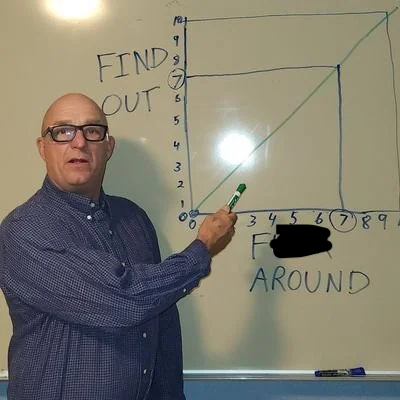
\includegraphics[width=0.6\textwidth,height=0.7\textheight]{figs/fafo.png}
\end{frame}

\begin{frame}{Can betting markets help us predict elections?}
\phantomsection\label{can-betting-markets-help-us-predict-elections}
\pause

\begin{itemize}
\tightlist
\item
  Data from an online betting company Intrade \pause
\item
  People trade contracts such as ``Obama to win the electoral votes in
  Florida'\,' \pause
\item
  Market prices of each contract fluctuate based on its sales \pause
\item
  Why might we expect betting markets like Intrade to accurately predict
  outcomes of elections?
\end{itemize}
\end{frame}

\begin{frame}{Linear Regression: Prediction using bivariate
relationships}
\phantomsection\label{linear-regression-prediction-using-bivariate-relationships}
\pause

\begin{itemize}
\tightlist
\item
  Goal: what's our best guess about \(Y_i\) if we know what \(X_i\) is?
  \pause

  \begin{itemize}
  \tightlist
  \item
    What's our best guess about election margins if we know the market's
    margins? \pause
  \end{itemize}
\item
  Terminology:

  \begin{itemize}
  \tightlist
  \item
    \textbf{Dependent/outcome variable}: what we want to predict
    (election margin). \pause
  \item
    \textbf{Independent/explanatory variable}: what we're using to
    predict (market margin).
  \end{itemize}
\end{itemize}
\end{frame}

\begin{frame}[fragile]{We'll use two datasets: \texttt{intrade08.csv} \&
\texttt{pres08.csv}}
\phantomsection\label{well-use-two-datasets-intrade08.csv-pres08.csv}
\footnotesize

\begin{longtable}[]{@{}
  >{\raggedright\arraybackslash}p{(\columnwidth - 2\tabcolsep) * \real{0.1495}}
  >{\raggedright\arraybackslash}p{(\columnwidth - 2\tabcolsep) * \real{0.8505}}@{}}
\toprule\noalign{}
\begin{minipage}[b]{\linewidth}\raggedright
Name
\end{minipage} & \begin{minipage}[b]{\linewidth}\raggedright
Description
\end{minipage} \\
\midrule\noalign{}
\endhead
\texttt{day} & Date of the session \\
\texttt{statename} & Full name of each state (including DC in 2008) \\
\texttt{state} & Abbreviation of each state (including DC in 2008) \\
\texttt{PriceD} & Closing price (predicted vote share) of Democratic
Nominee's market \\
\texttt{PriceR} & Closing price (predicted vote share) of Republican
Nominee's market \\
\texttt{VolumeD} & Total session trades of Democratic Party Nominee's
market \\
\texttt{VolumeR} & Total session trades of Republican Party Nominee's
market \\
\bottomrule\noalign{}
\end{longtable}

\begin{itemize}
\tightlist
\item
  \texttt{intrade08.csv}: Each row represents daily trading information
  about the contracts for either the Democratic or Republican Party
  nominee's victory in a particular state.
\end{itemize}
\end{frame}

\begin{frame}[fragile]{Presidential voting data from 2008}
\phantomsection\label{presidential-voting-data-from-2008}
\begin{longtable}[]{@{}
  >{\raggedright\arraybackslash}p{(\columnwidth - 2\tabcolsep) * \real{0.2593}}
  >{\raggedright\arraybackslash}p{(\columnwidth - 2\tabcolsep) * \real{0.7284}}@{}}
\toprule\noalign{}
\begin{minipage}[b]{\linewidth}\raggedright
Name
\end{minipage} & \begin{minipage}[b]{\linewidth}\raggedright
Description
\end{minipage} \\
\midrule\noalign{}
\endhead
\texttt{state.name} & Full name of state (only in \texttt{pres2008}) \\
\texttt{state} & Two letter state abbreviation \\
\texttt{Obama} & Vote percentage for Obama \\
\texttt{McCain} & Vote percentage for McCain \\
\texttt{EV} & Number of electoral college votes for this state \\
\bottomrule\noalign{}
\end{longtable}
\end{frame}

\begin{frame}[fragile]{Predicting Elections Using Betting Markets and
Linear Models}
\phantomsection\label{predicting-elections-using-betting-markets-and-linear-models}
\pause

\begin{itemize}
\tightlist
\item
  Load the data
\end{itemize}

\begin{Shaded}
\begin{Highlighting}[]
\FunctionTok{library}\NormalTok{(tidyverse)}
\NormalTok{intrade08 }\OtherTok{\textless{}{-}} \FunctionTok{read.csv}\NormalTok{(}\StringTok{"../data/intrade08.csv"}\NormalTok{)}
\NormalTok{pres08 }\OtherTok{\textless{}{-}} \FunctionTok{read.csv}\NormalTok{(}\StringTok{"../data/pres08.csv"}\NormalTok{)}

\DocumentationTok{\#\# merge datasets and calculate margins for DV and IV}
\NormalTok{intresults08 }\OtherTok{\textless{}{-}} \FunctionTok{inner\_join}\NormalTok{(intrade08,pres08) }\SpecialCharTok{\%\textgreater{}\%}
  \FunctionTok{mutate}\NormalTok{(}\AttributeTok{obama.intmarg =}\NormalTok{ PriceD }\SpecialCharTok{{-}}\NormalTok{ PriceR,}
         \AttributeTok{obama.actmarg =}\NormalTok{ Obama }\SpecialCharTok{{-}}\NormalTok{ McCain)}
\end{Highlighting}
\end{Shaded}
\end{frame}

\begin{frame}{Plot bivariate relationship}
\phantomsection\label{plot-bivariate-relationship}
\begin{center}\includegraphics{psc7475_lecture_5_slides_files/figure-beamer/unnamed-chunk-23-1} \end{center}
\end{frame}

\begin{frame}{Using a line to predict}
\phantomsection\label{using-a-line-to-predict}
\pause

\begin{itemize}
\tightlist
\item
  Prediction: for any value of \(X\) , what's the best guess about
  \(Y\)? \pause

  \begin{itemize}
  \tightlist
  \item
    Need a function \(y = f(x)\) that maps values of \(X\) into
    predictions. \pause
  \item
    \textbf{Machine learning}: fancy ways to determine \(f(x)\) \pause
  \end{itemize}
\item
  Simplest possible way to relate two variables: a line. \pause
\end{itemize}

\[  
y = mx + b
\]

\pause

\begin{itemize}
\tightlist
\item
  Problem: for any line we draw, not all the data is on the line. \pause

  \begin{itemize}
  \tightlist
  \item
    Some points will be above the line, some below. \pause
  \item
    Need a way to account for \textbf{chance variation} away from the
    line.
  \end{itemize}
\end{itemize}
\end{frame}

\begin{frame}{Linear Regression Model}
\phantomsection\label{linear-regression-model}
\begin{itemize}
\tightlist
\item
  Model for the line of best fit
\end{itemize}

\[
Y_i = \underbrace{\alpha}_{\textrm{intercept}} + \underbrace{\beta}_{\textrm{slope}} \times X_i + \underbrace{\epsilon_i}_{\textrm{error term}}
\] \pause

\begin{itemize}
\tightlist
\item
  \textbf{Coefficients/parameters} \((\alpha,\beta)\): true unknown
  intercept/slope of the line of best fit \pause
\item
  \textbf{Chance error} \((\epsilon_i)\): accounts for the fact that the
  line doesn't perfectly fit the data. \pause

  \begin{itemize}
  \tightlist
  \item
    Each observation allowed to be off the regression line
  \item
    Chance errors are 0 on average \pause
  \end{itemize}
\item
  Useful fiction: this model represents the \textbf{data generating
  process}

  \begin{itemize}
  \tightlist
  \item
    George Box: ``all models are wrong, some are useful''
  \end{itemize}
\end{itemize}
\end{frame}

\begin{frame}{Interpretting the Regression Line}
\phantomsection\label{interpretting-the-regression-line}
\[
Y_i = \alpha + \beta \times X_i + \epsilon_i
\]

\pause

\begin{itemize}
\tightlist
\item
  \textbf{Intercept} \(alpha\): average value of \(Y\) when \(X\) is 0

  \begin{itemize}
  \tightlist
  \item
    Average Obama margin when market's margin is 0. \pause
  \end{itemize}
\item
  \textbf{Slope} \(\beta\): average change in \(Y\) when \(X\) increases
  by one unit

  \begin{itemize}
  \tightlist
  \item
    Average increase in Obama margin for each additional margin increase
    by the market. \pause
  \end{itemize}
\item
  But we don't know \(\alpha\) or \(\beta\). How can we estimate them?
  Next time\ldots{} \pause

  \begin{itemize}
  \tightlist
  \item
    Or now if we still have time!
  \end{itemize}
\end{itemize}
\end{frame}

\begin{frame}{Linear Regression Model (skip if same day)}
\phantomsection\label{linear-regression-model-skip-if-same-day}
\begin{itemize}
\tightlist
\item
  Model for the line of best fit
\end{itemize}

\[
Y_i = \underbrace{\alpha}_{\textrm{intercept}} + \underbrace{\beta}_{\textrm{slope}} \times X_i + \underbrace{\epsilon_i}_{\textrm{error term}}
\]

\begin{itemize}
\tightlist
\item
  \textbf{Coefficients/parameters} \((\alpha,\beta)\): true unknown
  intercept/slope of the line of best fit
\item
  \textbf{Chance error} \((\epsilon_i)\): accounts for the fact that the
  line doesn't perfectly fit the data.

  \begin{itemize}
  \tightlist
  \item
    Each observation allowed to be off the regression line
  \item
    Chance errors are 0 on average
  \end{itemize}
\end{itemize}
\end{frame}

\begin{frame}{Estimate coefficients}
\phantomsection\label{estimate-coefficients}
\pause

\begin{itemize}
\tightlist
\item
  Parameters: \(\alpha, \beta\)

  \begin{itemize}
  \tightlist
  \item
    Unknown features of the data-generating process.
  \item
    Chance error makes these impossible to observe directly. \pause
  \end{itemize}
\item
  Estimates: \(\hat{\alpha}, \hat{\beta}\)

  \begin{itemize}
  \tightlist
  \item
    An estimate is our best guess about some parameter. \pause
  \end{itemize}
\item
  Regression line:
\end{itemize}

\[
\hat{Y} = \hat{\alpha} + \hat{\beta} * x
\]

\begin{itemize}
\tightlist
\item
  Average value of \(Y\) when \(X\) is \(x\)
\item
  Represents the best guess or \textbf{predicted value} of the outcome
  at \(x\).
\end{itemize}
\end{frame}

\begin{frame}{Line of best fit}
\phantomsection\label{line-of-best-fit}
\begin{center}\includegraphics{psc7475_lecture_5_slides_files/figure-beamer/unnamed-chunk-24-1} \end{center}
\end{frame}

\begin{frame}{Why not this line?}
\phantomsection\label{why-not-this-line}
\begin{center}\includegraphics{psc7475_lecture_5_slides_files/figure-beamer/unnamed-chunk-25-1} \end{center}
\end{frame}

\begin{frame}{Least squares}
\phantomsection\label{least-squares}
\pause

\begin{itemize}
\tightlist
\item
  How do we figure out the best line to draw? \pause

  \begin{itemize}
  \tightlist
  \item
    \textbf{Fitted/predicted value} for each observation:
    \(\hat{Y} = \hat{\alpha} + \hat{beta} \times X_i\) \pause
  \item
    \textbf{Residual/prediction error}:
    \(\hat{\epsilon_i} = Y_i - \hat{Y}\) \pause
  \end{itemize}
\item
  Get these estimates by the \textbf{least squares method} \pause
\item
  Minimize the \textbf{sum of the squared residuals} (SSR): \pause
\end{itemize}

\[
SSR = \sum_{i=1}^{n} \hat{\epsilon}_i^2 = \sum_{i=1}^n (Y_i - \hat{\alpha} - \hat{\beta}X_i)^2
\]

\pause

\begin{itemize}
\tightlist
\item
  Finds the line that minimizes the magnitude of the prediction errors!
\end{itemize}
\end{frame}

\begin{frame}[fragile]{Linear Regression in R}
\phantomsection\label{linear-regression-in-r}
\pause

\begin{itemize}
\tightlist
\item
  R will calculate least squares line for a data set using \texttt{lm()}
  \pause

  \begin{itemize}
  \tightlist
  \item
    Syntax: \texttt{lm(y\ \textasciitilde{}\ x,\ data\ =\ mydata)}
    \pause
  \item
    \texttt{y} is the name of the dependent variable
  \item
    \texttt{x} is the name of the independent variable
  \item
    \texttt{mydata} is the data.frame where they live
  \end{itemize}
\end{itemize}
\end{frame}

\begin{frame}[fragile]{Linear Regression in R}
\phantomsection\label{linear-regression-in-r-1}
\small

\begin{Shaded}
\begin{Highlighting}[]
\NormalTok{fit }\OtherTok{\textless{}{-}} \FunctionTok{lm}\NormalTok{(obama.actmarg }\SpecialCharTok{\textasciitilde{}}\NormalTok{ obama.intmarg, }\AttributeTok{data =}\NormalTok{ intresults08)}
\NormalTok{fit}
\end{Highlighting}
\end{Shaded}

\begin{verbatim}
## 
## Call:
## lm(formula = obama.actmarg ~ obama.intmarg, data = intresults08)
## 
## Coefficients:
##   (Intercept)  obama.intmarg  
##        5.5681         0.2799
\end{verbatim}
\end{frame}

\begin{frame}[fragile]{Coefficients and fitted values}
\phantomsection\label{coefficients-and-fitted-values}
\begin{itemize}
\tightlist
\item
  Use \texttt{coef()} to extract estimated coefficients:
\end{itemize}

\begin{Shaded}
\begin{Highlighting}[]
\FunctionTok{coef}\NormalTok{(fit)}
\end{Highlighting}
\end{Shaded}

\begin{verbatim}
##   (Intercept) obama.intmarg 
##     5.5681423     0.2799326
\end{verbatim}

\begin{itemize}
\tightlist
\item
  R can show you each of the fitted values as well:
\end{itemize}

\begin{Shaded}
\begin{Highlighting}[]
\FunctionTok{head}\NormalTok{(}\FunctionTok{fitted}\NormalTok{(fit))}
\end{Highlighting}
\end{Shaded}

\begin{verbatim}
##        1        2        3        4        5        6 
## 5.568142 5.568142 5.568142 5.568142 5.568142 5.568142
\end{verbatim}
\end{frame}

\begin{frame}{Properties of least squares}
\phantomsection\label{properties-of-least-squares}
\begin{itemize}
\tightlist
\item
  Least squares line always goes through \((\bar{X},\bar{Y})\)
\item
  Estimated slope is related to correlation:
\end{itemize}

\[
\hat{\beta} = (\textrm{correlation of } X \textrm{and } Y) \times \frac{\textrm{SD of }Y}{\textrm{SD of }X}
\]

\begin{itemize}
\tightlist
\item
  Mean of residuals is always 0
\end{itemize}
\end{frame}

\begin{frame}{Visual components of least squares}
\phantomsection\label{visual-components-of-least-squares}
\begin{center}\includegraphics{psc7475_lecture_5_slides_files/figure-beamer/unnamed-chunk-29-1} \end{center}
\end{frame}

\begin{frame}{Visual components of least squares}
\phantomsection\label{visual-components-of-least-squares-1}
\begin{center}\includegraphics{psc7475_lecture_5_slides_files/figure-beamer/unnamed-chunk-30-1} \end{center}
\end{frame}

\begin{frame}{Visual components of least squares}
\phantomsection\label{visual-components-of-least-squares-2}
\begin{center}\includegraphics{psc7475_lecture_5_slides_files/figure-beamer/unnamed-chunk-31-1} \end{center}
\end{frame}

\end{document}
